\begin{enumerate}[label=\thechapter.\arabic*,ref=\thechapter.\theenumi]
\item A damper with damping coefficient, $c$, is attached to a mass of $5$ \text{kg} and spring of stiffness  $5$ \text{kN/m} as shown in figure. The system undergoes under-damped oscillations.
If the ratio of the $3^{rd}$ amplitude to the $4^{th}$ amplitude of oscillations is ${1.5}$, the value of $c$ is ?
\begin{figure}[ht]
    \centering
    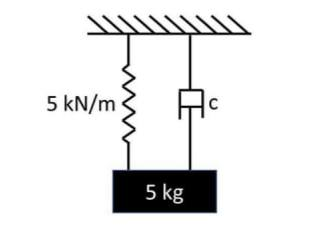
\includegraphics[width=\columnwidth]{2022/AE/62/figs/fig1.png}
\end{figure}

\hfill {(GATE AE-62 (2022))}
\solution
\iffalse
\let\negmedspace\undefined
\let\negthickspace\undefined
\documentclass[journal,12pt,twocolumn]{IEEEtran}
\usepackage{cite}
\usepackage{amsmath,amssymb,amsfonts,amsthm}
\usepackage{algorithmic}
\usepackage{graphicx}
\usepackage{textcomp}
\usepackage{xcolor}
\usepackage{txfonts}
\usepackage{listings}
\usepackage{enumitem}
\usepackage{mathtools}
\usepackage{gensymb}
\usepackage[breaklinks=true]{hyperref}
\usepackage{tkz-euclide} % loads  TikZ and tkz-base
\usepackage{listings}
\usepackage{gvv}
\usepackage{circuitikz}
\newtheorem{theorem}{Theorem}[section]
\newtheorem{problem}{Problem}
\newtheorem{proposition}{Proposition}[section]
\newtheorem{lemma}{Lemma}[section]
\newtheorem{corollary}[theorem]{Corollary}
\newtheorem{example}{Example}[section]
\newtheorem{definition}[problem]{Definition}
%\newtheorem{thm}{Theorem}[section] 
%\newtheorem{defn}[thm]{Definition}
%\newtheorem{algorithm}{Algorithm}[section]
%\newtheorem{cor}{Corollary}
\newcommand{\BEQA}{\begin{eqnarray}}
\newcommand{\EEQA}{\end{eqnarray}}
\newcommand{\define}{\stackrel{\triangle}{=}}
\theoremstyle{remark}
\newtheorem{rem}{Remark}

%\bibliographystyle{ieeetr}
\begin{document}
%

\bibliographystyle{IEEEtran}


\vspace{3cm}

\title{
%  \logo{
GATE AE-62 (2022)

\large{EE:1205 \brak{Signals Systems}}

Indian Institute of Technology, Hyderabad
%  }
}
\author{Md Ayaan Ashraf

EE23BTECH11041
}  
\maketitle
\newpage
\bigskip
\renewcommand{\thefigure}{\arabic{figure}}
\renewcommand{\thetable}{\arabic{table}}
%\renewcommand{\theequation}{\theenumi}
\section*{\textit{\textbf{Question}}}
A damper with damping coefficient, $c$, is attached to a mass of $5$ \text{kg} and spring of stiffness  $5$ \text{kN/m} as shown in figure. The system undergoes under-damped oscillations.
If the ratio of the $3^{rd}$ amplitude to the $4^{th}$ amplitude of oscillations is ${1.5}$, the value of $c$ is ?
\begin{figure}[ht]
    \centering
    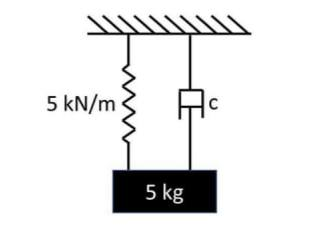
\includegraphics[width=\columnwidth]{2022/AE/62/figs/fig1.png}
\end{figure}

\hfill {(GATE AE-62 (2022))}
\section*{\textit{\textbf{Solution:}}}
\fi

\begin{table}[ht]
  \begin{tabular}{|c||c||c|}
    \hline
    \textbf{Parameter} & \textbf{Value} & \textbf{Description} \\
    \hline
    $c$ & $? $ & Damping Coefficient \\
    \hline
    $k$ & $5$ \text{kN/m} & Stiffness \\
    \hline
    $r$ & $1.5$ & Ratio of $3^{rd}$ amplitude to $4^{th}$ \\&& amplitude of oscillations \\
    \hline
  \end{tabular}
  \vspace{2mm}
  \caption{Parameter Table (GATE AE-62)}
\end{table}


    \begin{figure}[h]
        \centering
        
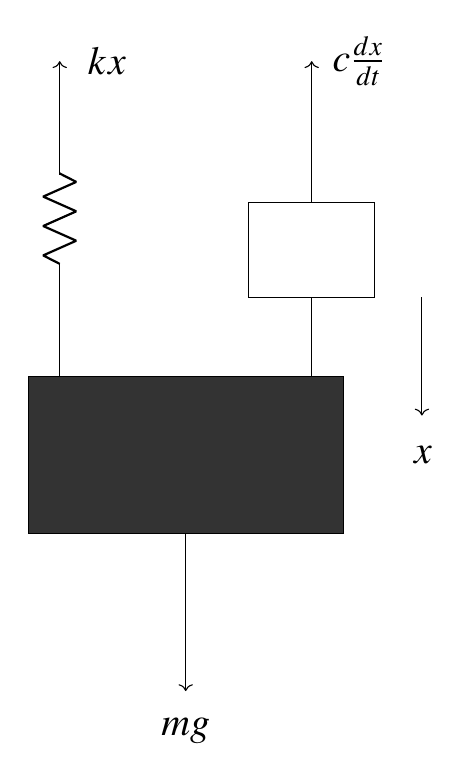
\begin{tikzpicture}[scale=1]
\draw (0,0) rectangle (4,2);
  \filldraw[fill=black!80] (0,0) rectangle (4,2);
\draw (0.4,2) -- (0.4,3);
% \draw[decorate,decoration={coil,amplitude=6pt,segment length=7pt}] (0.4,3) -- (0.4,5);
\draw (0.4,3) to [R] (0.4,5);
\draw [->](0.4,5)--(0.4,6);
\draw (3.6,2) -- (3.6,3);
\draw (2.8,3) rectangle (4.4,4.2);
\draw [->](3.6,4.2)--(3.6,6);

 \node at (4.2,6) {\Large$c\frac{dx}{dt}$};
 \node at (1,6) {\Large$kx$}; 
 \draw[->] (5,3)  -- (5,1.5);
 \node at (5,1) {\Large $x$};

 \draw[->](2,0) -- (2,-2);
 \node at (2,-2.5) {\Large$mg$};
\end{tikzpicture}


        \label{fig:Fig-1}
    \end{figure}
    Now, as the oscillation begins, from the \figref{fig:Fig-1} we write net force on the mass as,
    \begin{align}
        &F=F_{1}+F_{2}+mgu(t) \label{eq:3}\\
        \implies &m\frac{d^2x(t)}{dt^2}=-kx(t)-c\frac{dx(t)}{dt}+mgu(t) \label{eq:4}\\
        \implies &\frac{d^2x(t)}{dt^2}+\brak{\frac{c}{m}}\frac{dx(t)}{dt}+\brak{\frac{k}{m}}x(t)=gu(t) \label{eq:5}
    \end{align}

    Now, taking the Laplace transform on both sides,
    \begin{align}
        &s^2X(s)+\frac{c}{m}sX(s)+\frac{k}{m}X(s)=\frac{g}{s} \label{eq:6}\\
        \implies &X(s)=\frac{g}{s\brak{s^2+\frac{c}{m}s+\frac{k}{m}}} \label{eq:7}\\
        \implies &X(s)=\frac{g}{s(s-s_1)(s-s_2)} \label{eq:8}
    \end{align}
    Where
    \begin{align}
        &s_1=-\frac{c}{2m}+\sqrt{\brak{\frac{c}{2m}}^2-\frac{k}{m}} \label{eq:9}\\
        &s_2=-\frac{c}{2m}-\sqrt{\brak{\frac{c}{2m}}^2-\frac{k}{m}} \label{eq:10}
    \end{align}
    From \eqref{eq:8} we get,
    \begin{align}
        \begin{split}
            \implies &X(s)=\frac{g}{(s_1-s_2)}\sbrak{\frac{1}{s_1(s-s_1)}-\frac{1}{s_2(s-s_2)}} \\
            &-\frac{g}{s_1s_2}\brak{\frac{1}{s}} \label{eq:11}
        \end{split}
    \end{align}
    Now again taking the inverse Laplace transform we have,
    \begin{align}
        &x(t)=-\frac{g}{s_1s_2}u(t)+\frac{g}{(s_1-s_2)}\sbrak{\frac{1}{s_1}e^{s_1t}-\frac{1}{s_2}e^{s_2t}}u(t)\label{eq:12}
    \end{align}
    \begin{align}
    \begin{split}
    \implies &x(t) = -\sqrt{\brak{\frac{mg}{k}}^2 + \brak{\frac{gc}{2mk}}^2}e^{-ct/2m}u(t) \\
            &\sin{\brak{\sqrt{\frac{k}{m} - \brak{\frac{c}{2m}}^2}t + \tan^{-1}\brak{\frac{2mg\sqrt{\frac{k}{m} - \brak{\frac{c}{2m}}^2}}{gc}}}} \\
            &- \frac{mg}{k}
        u(t) \label{eq:13}
\end{split}
\end{align}
    (Substituting the values of $s_1$ and $s_2$ from \eqref{eq:9} and \eqref{eq:10})

    From \eqref{eq:13}, we have the ratio of $3^{rd}$ to $4^{th}$ amplitude,
    \begin{align}
        \begin{split}
            &-\sqrt{\brak{\frac{mg}{k}}^2+\brak{\frac{gc}{2mk}}^2}e^{-3cT/2m}= \\
            &-\frac{3}{2}\sqrt{\brak{\frac{mg}{k}}^2+\brak{\frac{gc}{2mk}}^2}e^{-4cT/2m} \label{eq:14}
        \end{split}
    \end{align}
    \begin{align}
        \implies &e^{\pi c/\sqrt{mk}}=\frac{3}{2} \label{eq:15}\\
        \implies &c=\frac{\sqrt{mk}\ln{\frac{3}{2}}}{\pi} \label{eq:16}
    \end{align}
\begin{figure}[h!]
    \centering
    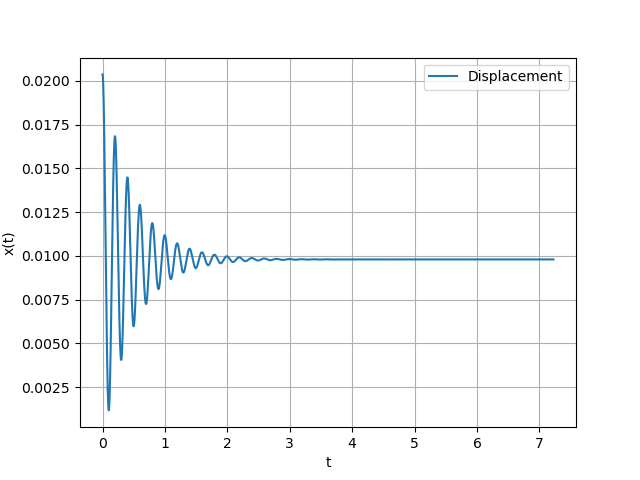
\includegraphics[width=\columnwidth]{2022/AE/62/figs/fig2.png}
\end{figure}




\newpage
\item A spring-mass system having a mass $m$ and spring constant $k$, placed horizontally on a foundation, is connected to a vertically hanging mass $m$ with the help of an inextensible string. Ignore the friction in the pulleys and also the inertia of pulleys, string and spring. Gravity is acting vertically downward as shown. The natural frequency of the system in rad/s is 
\begin{figure}[htbp]
	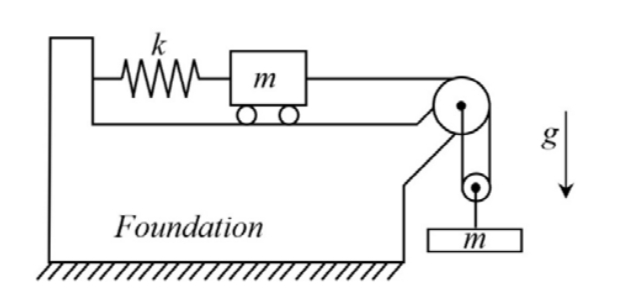
\includegraphics[width=\columnwidth]{2022/XE/76/figs/question_xe76_22.jpg}
	\label{fig:question_xe76_22}
\end{figure}
\begin{enumerate}[label=(\Alph*)]
\item $\sqrt{\frac{4k}{3m}}$
\item $\sqrt{\frac{k}{2m}}$
\item $\sqrt{\frac{k}{3m}}$
\item $\sqrt{\frac{4k}{5m}}$
\end{enumerate}
\hfill(GATE XE 2022)
\\
\solution
\iffalse
\let\negmedspace\undefined
\let\negthickspace\undefined
\documentclass[journal,12pt,twocolumn]{IEEEtran}
\usepackage{cite}
\usepackage{amsmath,amssymb,amsfonts,amsthm}
\usepackage{algorithmic}
\usepackage{graphicx}
\usepackage{textcomp}
\usepackage{xcolor}
\usepackage{txfonts}
\usepackage{listings}
\usepackage{enumitem}
\usepackage{mathtools}
\usepackage{gensymb}
\usepackage{comment}
\usepackage[breaklinks=true]{hyperref}
\usepackage{tkz-euclide} 
\usepackage{listings}
\usepackage{gvv}                                        
\def\inputGnumericTable{}                                 
\usepackage[latin1]{inputenc}                                
\usepackage{color}                                            
\usepackage{array}                                            
\usepackage{longtable}                                       
\usepackage{calc}                                             
\usepackage{multirow}                                         
\usepackage{hhline}                                           
\usepackage{ifthen}                                           
\usepackage{lscape}
\newtheorem{theorem}{Theorem}[section]
\newtheorem{problem}{Problem}
\newtheorem{proposition}{Proposition}[section]
\newtheorem{lemma}{Lemma}[section]
\newtheorem{corollary}[theorem]{Corollary}
\newtheorem{example}{Example}[section]
\newtheorem{definition}[problem]{Definition}
\newcommand{\BEQA}{\begin{eqnarray}}
\newcommand{\EEQA}{\end{eqnarray}}
\newcommand{\define}{\stackrel{\triangle}{=}}
\theoremstyle{remark}
\newtheorem{rem}{Remark}
\begin{document}

\bibliographystyle{IEEEtran}
\vspace{3cm}

\title{GATE: XE - 76.2022}
\author{EE23BTECH11224 - Sri Krishna Prabhas Yadla$^{*}$% <-this % stops a space
}
\maketitle
\newpage
\bigskip

\renewcommand{\thefigure}{\arabic{figure}}
\renewcommand{\thetable}{\arabic{table}}


\vspace{3cm}
\textbf{Question:} A spring-mass system having a mass $m$ and spring constant $k$, placed horizontally on a foundation, is connected to a vertically hanging mass $m$ with the help of an inextensible string. Ignore the friction in the pulleys and also the inertia of pulleys, string and spring. Gravity is acting vertically downward as shown. The natural frequency of the system in rad/s is 
\begin{figure}[htbp]
	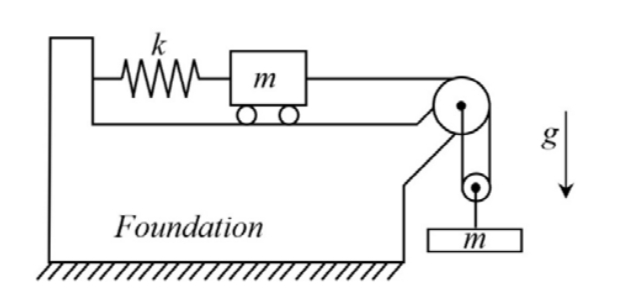
\includegraphics[width=\columnwidth]{2022/XE/76/figs/question_xe76_22.jpg}
	\label{fig:question_xe76_22}
\end{figure}
\begin{enumerate}[label=(\Alph*)]
\item $\sqrt{\frac{4k}{3m}}$
\item $\sqrt{\frac{k}{2m}}$
\item $\sqrt{\frac{k}{3m}}$
\item $\sqrt{\frac{4k}{5m}}$
\end{enumerate}
\hfill(GATE XE 2022)
\\
\solution
\fi
\begin{table}[htbp]
	\centering
	\def\arraystretch{1.5}
	\begin{tabular}{|c|p{4cm}|p{1.5cm}|}
\hline
\textbf{Parameters} & \textbf{Description} & \textbf{Value} \\
\hline
$x(t)$ & Displacement of mass $m$ on foundation at time $t$ & \\
\hline
$x(0)$ & Displacement of mass $m$ on foundation at time $t=0$ & 0 \\
\hline
$x'(0)$ & Velocity of mass $m$ on foundation at time $t=0$ & 0\\
\hline
\end{tabular}

	\caption{Parameters}
	\label{tab:parameters_xe76}
\end{table}
\begin{align}
T-kx &= m\frac{d^2x}{dt^2} \\
mg - 2T &= m\frac{d^2\brak{\frac{x}{2}}}{dt^2} \\
\implies mg - 2kx &= \frac{5}{2}m\frac{d^2x}{dt^2}\\
\label{xe76_L(x'')}\frac{d^2x}{dt^2} &\system{L} s^2X(s)-sx(0)-x'(0) \\
\label{xe76_L(t^n)}t^n &\system{L} \frac{n!}{s^{n+1}}
\end{align}
From the Laplace transforms \eqref{xe76_L(x'')} and \eqref{xe76_L(t^n)}, we get
\begin{align}
\frac{mg}{s}-2kX(s)&=\frac{5}{2}m\brak{s^2X(s)-sx(0)-x'(0)}\\
\implies X(s) &= \frac{\frac{2g}{5}}{s\brak{s^2+\frac{4k}{5m}}}\\
&= \frac{mg}{2ks}-\frac{mgs}{2k\brak{s^2+\frac{4k}{5m}}}\\
\label{xe76_L(cos{at})} \cos{at} &\system{L} \frac{s}{s^2+a^2}
\end{align}
From the Laplace transforms \eqref{xe76_L(t^n)} and \eqref{xe76_L(cos{at})}, we get
\begin{align}
x(t) &= \frac{mg}{2k}\brak{1-\cos{\brak{\sqrt{\frac{4k}{5m}}t}}}u(t)\\
\implies \omega &= \sqrt{\frac{4k}{5m}}
\end{align}
\begin{figure}[htbp]
	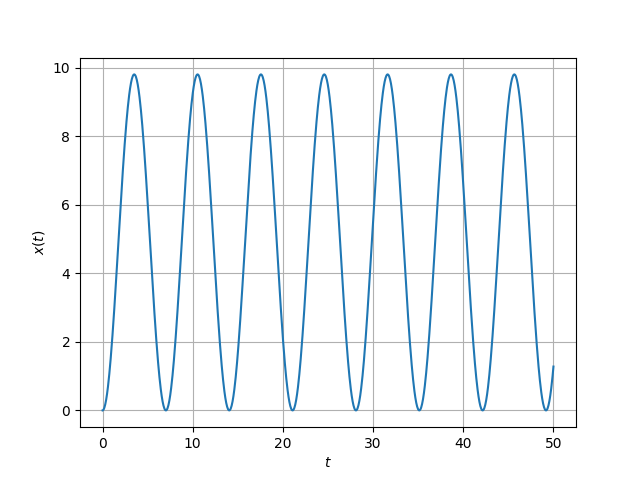
\includegraphics[width=\columnwidth]{2022/XE/76/figs/plot.png}
	\caption{Plot of $x(t)$ for $m=1kg$, $k=1N/m^2$}
	\label{fig:plot_xe76}
\end{figure}

\newpage

\item The time delay between the peaks of the voltage signals $ v_1\brak{t}= \cos\brak{{6t+60\degree}}$ and $ v_2\brak{t} = -\sin\brak{{6t}}$ is \rule{1cm}{0.15mm}s
\begin{enumerate}
    \item[(A)] $ \frac{300\pi}{360}$
    \item[(B)]$ \frac{10\pi}{360}$
    \item[(C)] $ \frac{50\pi}{360}$
    \item[(D)] $ \frac{200\pi}{360}$  
\end{enumerate}
\hfill(GATE BM 2022 QUESTION 18)\\
\solution
\iffalse
\let\negmedspace\undefined
\let\negthickspace\undefined
\documentclass[journal,12pt,twocolumn]{IEEEtran}
\usepackage{cite}
\usepackage{amsmath,amssymb,amsfonts,amsthm}
\usepackage{algorithmic}
\usepackage{graphicx}
\usepackage{textcomp}
\usepackage{xcolor}
\usepackage{txfonts}
\usepackage{listings}
\usepackage{enumitem}
\usepackage{mathtools}
\usepackage{gensymb}
\usepackage{comment}
\usepackage[breaklinks=true]{hyperref}
\usepackage{tkz-euclide}
\usepackage{listings}
\usepackage{gvv}
\def\inputGnumericTable{}
\usepackage[latin1]{inputenc}
\usepackage{color}
\usepackage{array}
\usepackage{longtable}
\usepackage{calc}
\usepackage{multirow}
\usepackage{hhline}
\usepackage{ifthen}
\usepackage{lscape}

\newtheorem{theorem}{Theorem}[section]
\newtheorem{problem}{Problem}
\newtheorem{proposition}{Proposition}[section]
\newtheorem{lemma}{Lemma}[section]
\newtheorem{corollary}[theorem]{Corollary}
\newtheorem{example}{Example}[section]
\newtheorem{definition}[problem]{Definition}
\newcommand{\BEQA}{\begin{eqnarray}}
\newcommand{\EEQA}{\end{eqnarray}}
\newcommand{\define}{\stackrel{\triangle}{=}}
\theoremstyle{remark}
\newtheorem{rem}{Remark}
\begin{document}

\bibliographystyle{IEEEtran}
\vspace{3cm}

\title{GATE 2022  -AE 63}
\author{EE23BTECH11057 - Shakunaveti Sai Sri Ram Varun$^{}$% &lt;-this % stops a space
}
\maketitle
\newpage
\bigskip
\vspace{2cm}
\textbf{Question: }
The time delay between the peaks of the voltage signals $ v_1\brak{t}= \cos\brak{{6t+60\degree}}$ and $ v_2\brak{t} = -\sin\brak{{6t}}$ is \rule{1cm}{0.15mm}s
\begin{enumerate}
    \item[(A)] $ \frac{300\pi}{360}$
    \item[(B)]$ \frac{10\pi}{360}$
    \item[(C)] $ \frac{50\pi}{360}$
    \item[(D)] $ \frac{200\pi}{360}$  
\end{enumerate}
\hfill(GATE BM 2022 QUESTION 18)\\
\textbf{Solution}:\\
\fi
\begin{table}[h!] 
\centering
\begin{tabular}{|c|c|c|}
    \hline
    \textbf{Parameter} & \textbf{Description} & \textbf{Value} \\
    \hline
    $v_1\brak{t}$ & Input voltage signal 1 & $ \cos\brak{{6t+60\degree}}$\\
    \hline
    $v_2\brak{t}$ & Input voltage signal 2 &$ -\sin\brak{{6t}}$ \\
    \hline
    $\Delta \phi$ & Phase difference between two input signals & ? \\
    \hline
    $\Delta t$ & Time difference between maxima of two input signals & ? \\
    \hline
    $\omega$ & angular frequency of input voltages& $ 6$\\
    \hline
\end{tabular}





\caption{input values}
\label{tab: Table2022bm18}
\end{table}
From the values given in the \tabref{tab: Table2022bm18}:
\begin{align}
v_1\brak{t} &= \cos\brak{{6t+60\degree}}\\ \label{eq: 2022bm181}
v_2\brak{t} &= -\sin{\brak{6t}}\\
\implies v_2\brak{t} &= \cos{\brak{6t + 90\degree}} \label{eq: 2022bm182}
\end{align}
From \eqref{eq: 2022bm181} and \eqref{eq: 2022bm182},
phase difference between two voltage signals is $ 30\degree$.
From formula,
\begin{align}
    \Delta \phi &= \frac{\Delta t}{\frac{2\pi}{\omega}}360\\
    \therefore \Delta t &= \frac{10\pi}{360}s
\end{align}
Hence, option B is correct.
\begin{figure}[h!]
    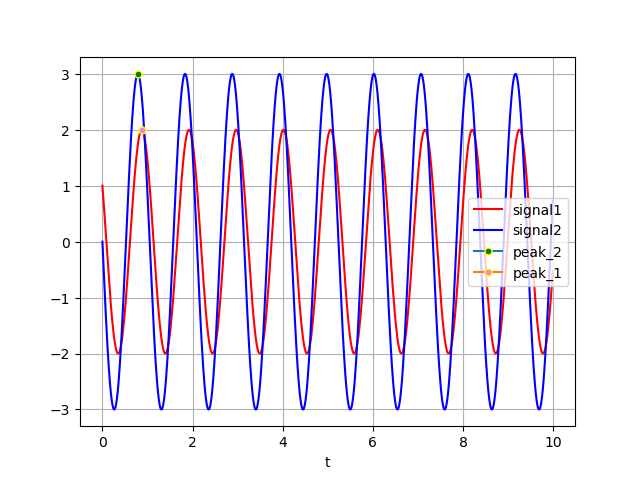
\includegraphics[width = 0.8\columnwidth]{2022/BM/18/figs/Figure_1.png}
    \caption{Figure of input voltage signals}
    \centering
    \label{fig: bm_18_2022}
\end{figure}



\item A sinusoidal carrier wave with amplitude $A_c$ and frequency $f_c$ is amplitude modulated with a message signal $m\brak{t}$ having frequency $0 < f_m << f_c$ to generate the modulated wave $s\brak{t}$ given by
$s\brak{t}$ = $A_c\brak{1 + m\brak{t}}cos (2\pi f_c t)$
The message signal that can be retrieved completely using
envelope detection is \underline{{\hspace{1.5in}}}
\begin{enumerate}
    \item $m\brak{t}= 0.5 \cos{\brak{2 \pi f_m t}}$
    \item $m\brak{t}= 1.5 \sin{\brak{2 \pi f_m t}}$
    \item $m\brak{t}= 2 \sin{\brak{4 \pi f_m t}}$
    \item $m\brak{t}= 2 \cos{\brak{4 \pi f_m t}}$
\end{enumerate}
\hfill(GATE IN 2022 QUESTION 16)\\
\solution\\
\iffalse
\let\negmedspace\undefined
\let\negthickspace\undefined
\documentclass[journal,12pt,twocolumn]{IEEEtran}
\usepackage{cite}
\usepackage{amsmath,amssymb,amsfonts,amsthm}
\usepackage{algorithmic}
\usepackage{graphicx}
\usepackage{textcomp}
\usepackage{xcolor}
\usepackage{txfonts}
\usepackage{listings}
\usepackage{enumitem}
\usepackage{mathtools}
\usepackage{gensymb}
\usepackage{comment}
\usepackage[breaklinks=true]{hyperref}
\usepackage{tkz-euclide} 
\usepackage{listings}
\usepackage{gvv}                                        
\def\inputGnumericTable{}                                 
\usepackage[latin1]{inputenc}                                
\usepackage{color}                                            
\usepackage{array}                                            
\usepackage{longtable}                                       
\usepackage{calc}                                             
\usepackage{multirow}                                         
\usepackage{hhline}                                           
\usepackage{ifthen}                                           
\usepackage{lscape}

\newtheorem{theorem}{Theorem}[section]
\newtheorem{problem}{Problem}
\newtheorem{proposition}{Proposition}[section]
\newtheorem{lemma}{Lemma}[section]
\newtheorem{corollary}[theorem]{Corollary}
\newtheorem{example}{Example}[section]
\newtheorem{definition}[problem]{Definition}
\newcommand{\BEQA}{\begin{eqnarray}}
\newcommand{\EEQA}{\end{eqnarray}}
\newcommand{\define}{\stackrel{\triangle}{=}}
\theoremstyle{remark}
\newtheorem{rem}{Remark}
\begin{document}
\bibliographystyle{IEEEtran}
\vspace{3cm}
\title{\textbf{IN-2022}}
\author{EE23BTECH11210-Dhyana Teja Machineni$^{*}$% <-this % stops a space
}
\maketitle
\newpage
\bigskip

\textbf{QUESTION:}\\
A sinusoidal carrier wave with amplitude $A_c$ and frequency $f_c$ is amplitude modulated with a message signal $m\brak{t}$ having frequency $0 < f_m << f_c$ to generate the modulated wave $s\brak{t}$ given by
$s\brak{t}$ = $A_c\brak{1 + m\brak{t}}cos (2\pi f_c t)$
The message signal that can be retrieved completely using
envelope detection is \underline{{\hspace{1.5in}}}
\begin{enumerate}
    \item $m\brak{t}= 0.5 \cos{\brak{2 \pi f_m t}}$
    \item $m\brak{t}= 1.5 \sin{\brak{2 \pi f_m t}}$
    \item $m\brak{t}= 2 \sin{\brak{4 \pi f_m t}}$
    \item $m\brak{t}= 2 \cos{\brak{4 \pi f_m t}}$
\end{enumerate}
\solution
\fi
\begin{table}[h]
         \label{tab:table}
         \renewcommand{\arraystretch}{1.5}
\begin{tabular}{|c|c|}
\hline
Parameter & Description  \\\hline
$s\brak{t}$& Amplitude Modulated Wave \\\hline
$M\brak{t}$ & Message Signal \\\hline
$c\brak{t}$ & Carrier Signal \\\hline
$f_c$ & Frequency of Carrier Signal\\\hline
$f_m$& Frequency of Message Signal \\ \hline
\end{tabular}

         \caption{Variables and their descriptions}
     \end{table}\\
\begin{align}
c\brak{t}&=A_c \cos\brak{2 \pi f_c t}\\
   M\brak{t}&= A_m \cos\brak{2 \pi f_m t}\\
    s\brak{t}&= \brak{A_c+ M\brak{t}} \cos\brak{2\pi f_c t}\\
    &=A_c\brak{1+\frac{A_m}{A_c} \cos\brak{2 \pi f_m t}}\cos{2 \pi f_c t}\\
    &=A_c\brak{1+m\brak{t}}\cos{2 \pi f_c t}
\end{align}
Modulation Index of $s\brak{t}=\mu= \frac{A_m}{A_c}$
\begin{itemize}
    \item $\mu<1$  Signal is Can be detected
    \item $\mu=1$   Signal Cannot be detected
    \item $\mu>1$   Over modualtion 
\end{itemize}
\begin{enumerate}

    \item m\brak{t} = 0.5 cos\brak{2 \pi f_m t} 
\begin{align}
    \frac{A_m}{A_c}= 0.5 \\
    \mu <1
\end{align}
$\therefore$ Signal can be retrieved completely.
\renewcommand{\thefigure}{\theenumi}
 \renewcommand{\thetable}{\theenumi}
\begin{figure}[h]
  
  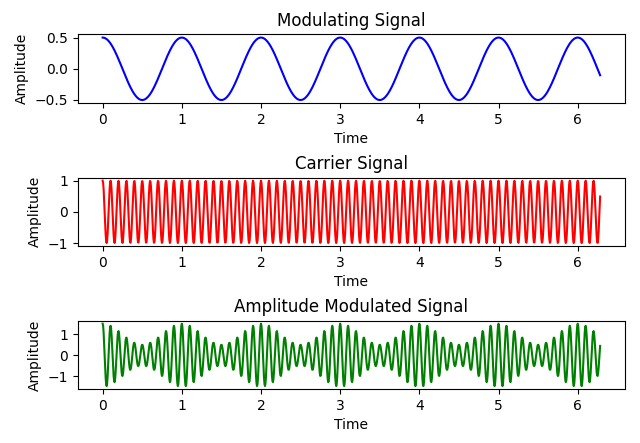
\includegraphics[width=\columnwidth]{2022/IN/16/figs/Figure_1.png}
  
\end{figure}
\item m\brak{t} = 1.5 sin\brak{2 \pi f_m t} 
\begin{align}
    \frac{A_m}{A_c}= 1.5\\
    \mu >1
\end{align}
$\therefore$ Signal cannot be retrieved completely.
\renewcommand{\thefigure}{\theenumi}
 \renewcommand{\thetable}{\theenumi}
\begin{figure}[h]
  
  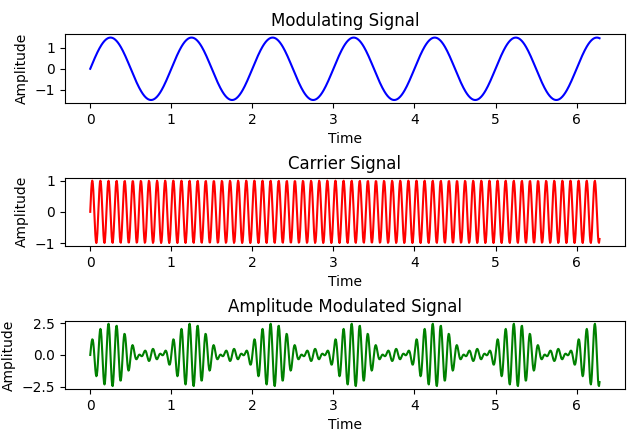
\includegraphics[width=\columnwidth]{2022/IN/16/figs/Figure_2.png}
  
\end{figure}
\item m\brak{t} = 2 sin\brak{4 \pi f_m t} 
\begin{align}
    \frac{A_m}{A_c}= 2\\
    \mu >1
\end{align}
$\therefore$ Signal cannot be retrieved completely.
\renewcommand{\thefigure}{\theenumi}
 \renewcommand{\thetable}{\theenumi}
\begin{figure}[h]
  
  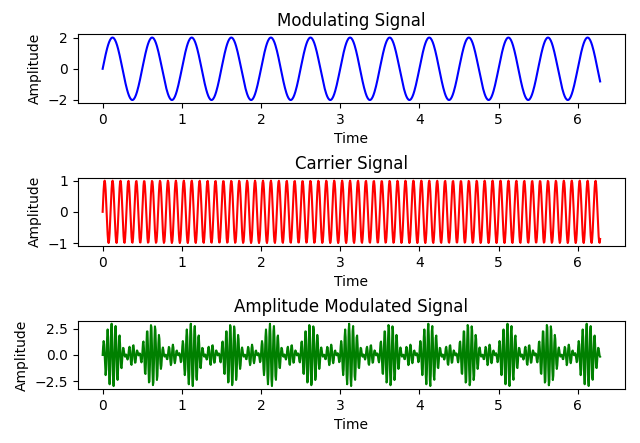
\includegraphics[width=\columnwidth]{2022/IN/16/figs/Figure_3.png}
  
\end{figure}
\item m\brak{t} = 2 cos\brak{4 \pi f_m t} 
\begin{align}
    \frac{A_m}{A_c}= 2\\
    \mu > 1
\end{align}
$\therefore$ Signal cannot be retrieved completely.
\renewcommand{\thefigure}{\theenumi}
 \renewcommand{\thetable}{\theenumi}
\begin{figure}[h]
  
  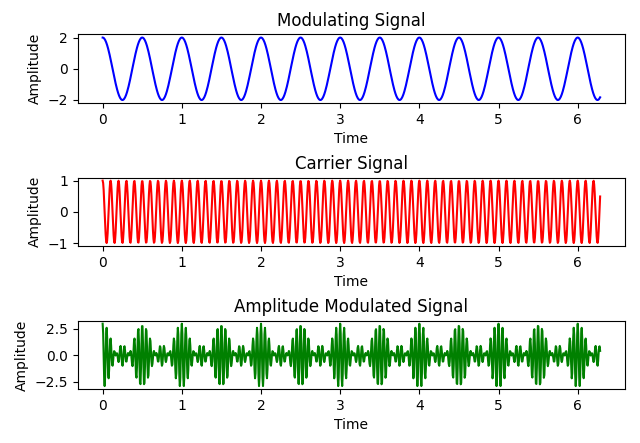
\includegraphics[width=\columnwidth]{2022/IN/16/figs/Figure_4.png}
  
\end{figure}
\end{enumerate}
 


\end{enumerate}
